\section{Transient analysis}
Transient analysis and simulations where done with the following simulation setup.
\begin{figure}[h!]
    \centering
    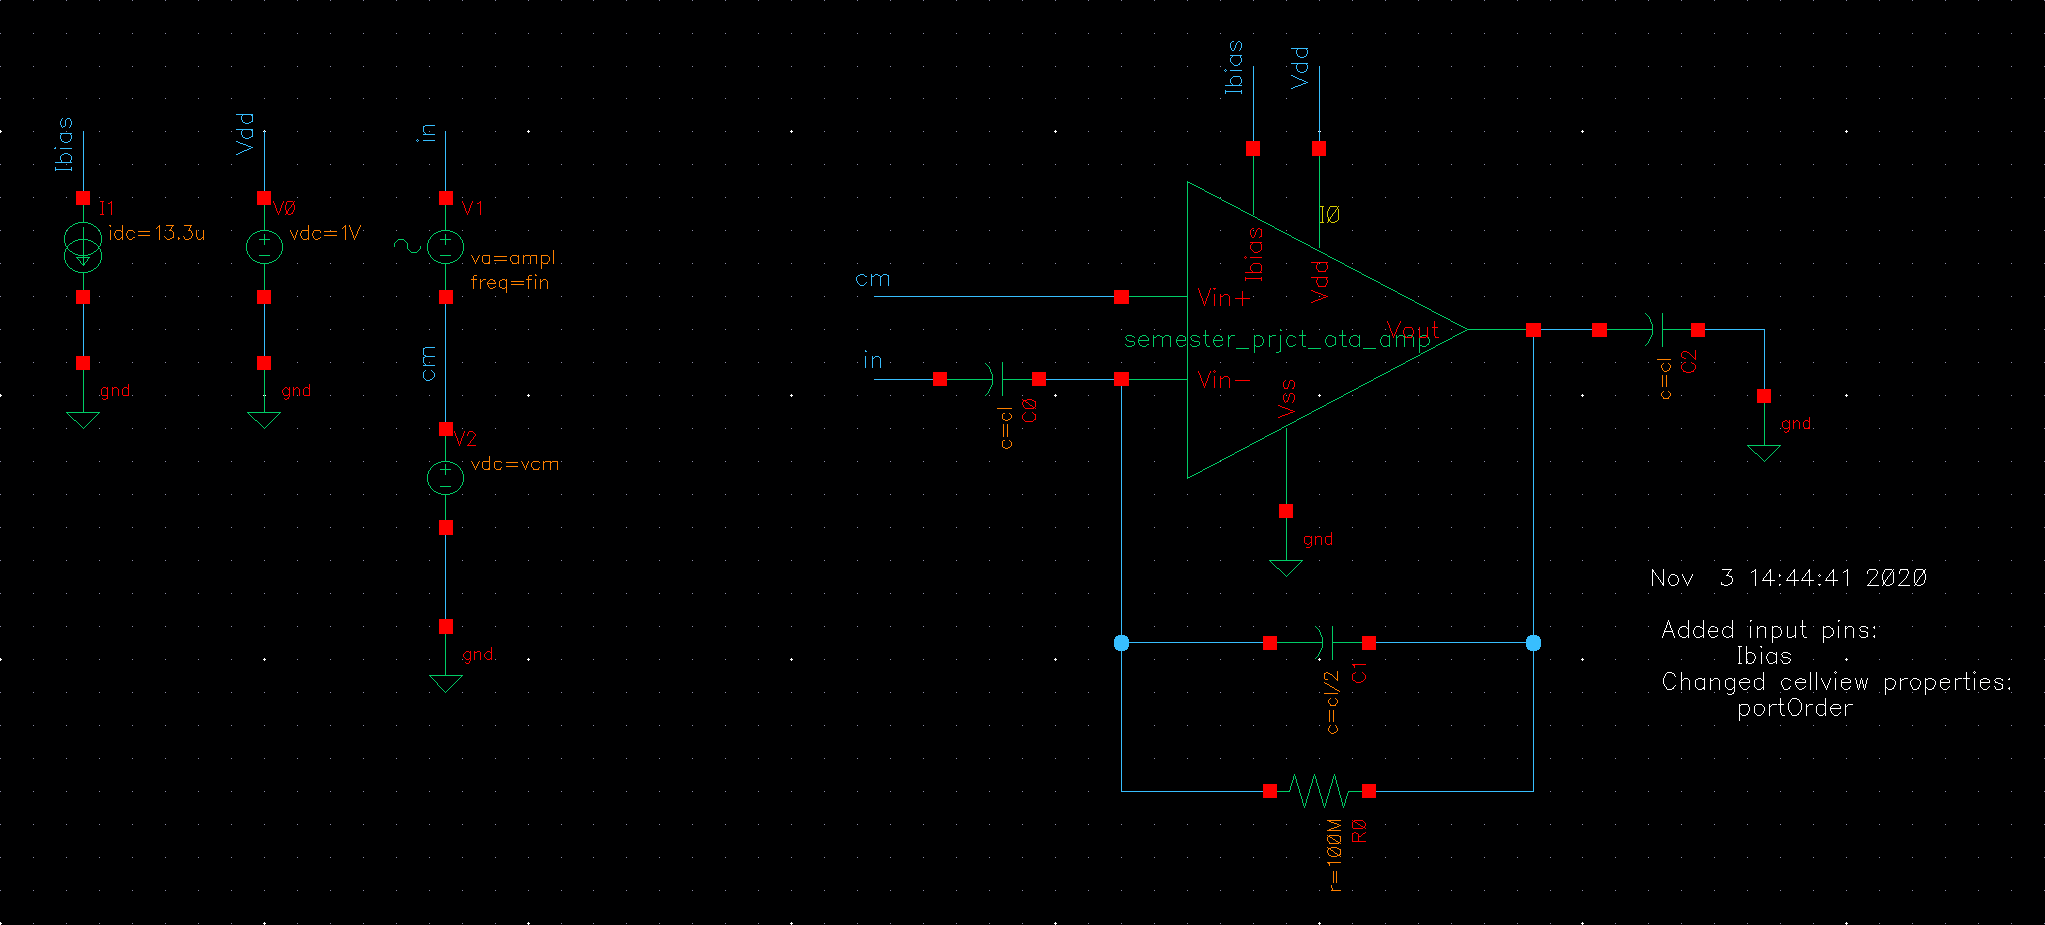
\includegraphics[width=.9\linewidth]{Images/Virtuoso/tran_tb.png}
    \caption{Transient testbench}
    \label{fig:trans:tb}
\end{figure}

\begin{figure}[h!]
    \centering
    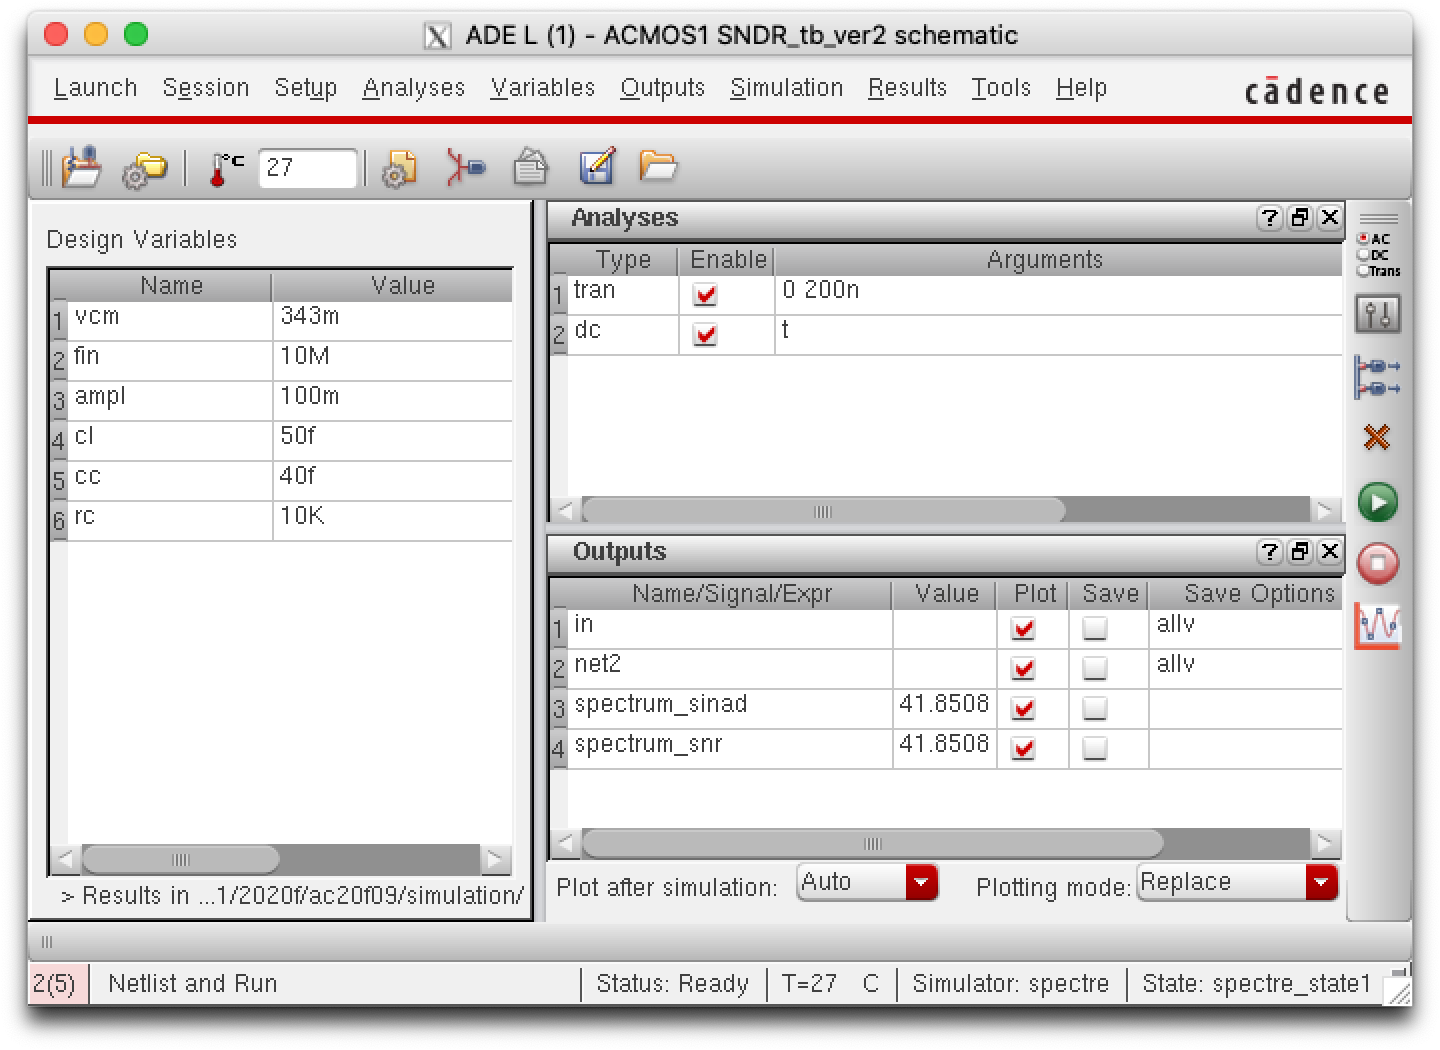
\includegraphics[width=.9\linewidth]{Images/Virtuoso/Transient_stimuli.png}
    \caption{ADE L setup for transient analysis}
    \label{fig:ADE:tran}
\end{figure}
As seen in figure \ref{fig:ADE:tran}, SNDR(SINAD) = 41.85 dB

\newpage
\null
\vfill
\begin{figure}[H]
    \centering
    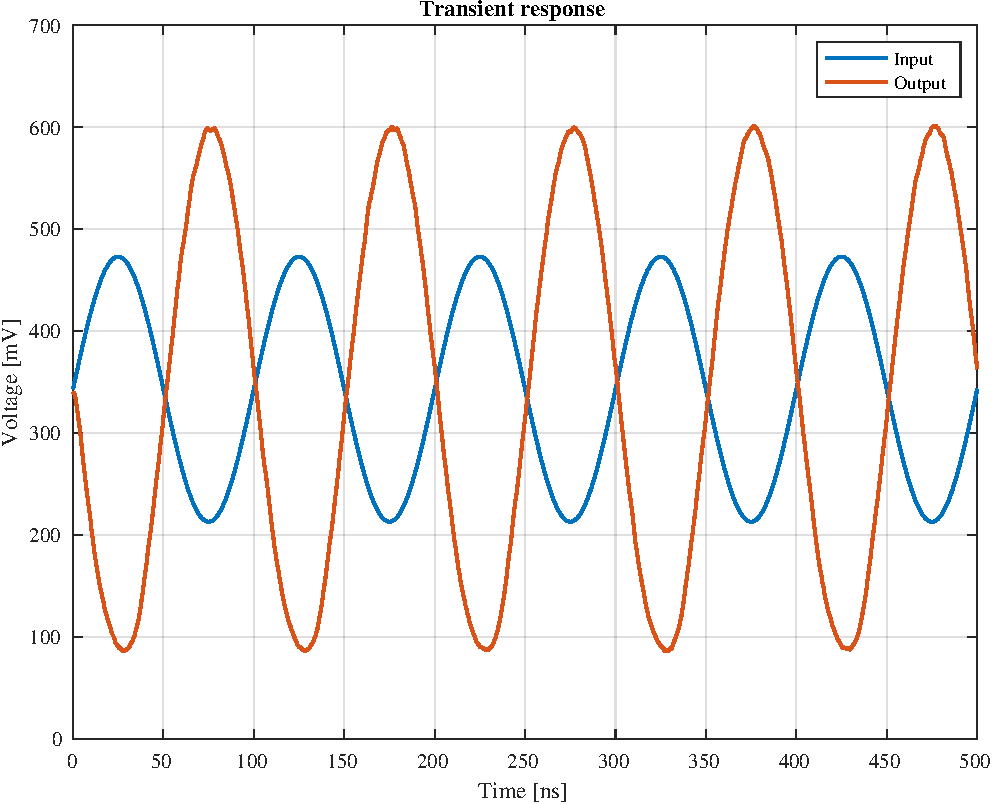
\includegraphics[width=.9\linewidth]{Images/Simulations/tran_response.pdf}
    \caption{Transient response}
    \label{fig:tran:sim}
\end{figure}
Figure \ref{fig:tran:sim} shows approximately \SI{0.5}{\volt} voltage swing at output. 
\vfill